\section{Deskripsi Sistem}
Sesuai dengan tujuan awal dari penelitian ini yaitu untuk membangun sistem \emph{question answering} data kabutapen di propinsi Nusa Tenggara Barat maka sistem akan dibangun berbasis web sehingga nantinya dapat diakses secara luas.

Aplikasi hanya memiliki satu buah halaman, dimana halaman ini terdiri dari form untuk melakukan input pertanyaan dalam bentuk kalimat tanya bahasa alami yang sesuai dengan tata bahasa Indonesia dan tombol untuk submit pertanyaan. Jawaban akan diberikan pada halaman yang sama. Secara umum, sistem \emph{question answering} yang akan dibangun terdiri dari tiga tahapan utama yaitu proses awal, proses utama dan proses akhir. Hal ini dapat dilihat pada gambar \ref{fig:gambaran_umum_sistem}.

\begin{figure}[th]
	\centering
	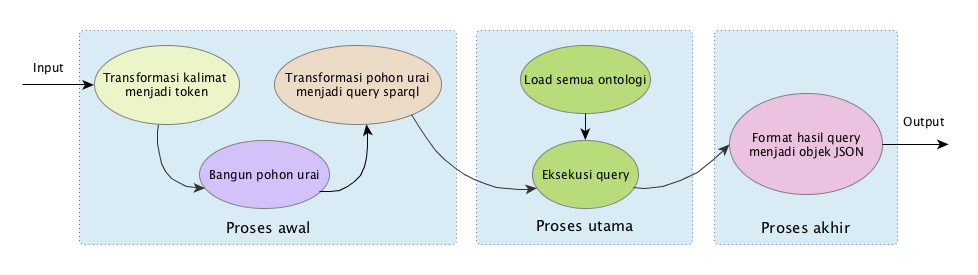
\includegraphics[width=1\textwidth]{gambaran_umum_sistem}
	\caption{Gambaran umum sistem}
	\label{fig:gambaran_umum_sistem}
\end{figure}

Proses awal berkaitan dengan pemrosesan kalimat tanya dimana proses ini merupakan proses transformasi bahasa alami menjadi pohon urai \emph{(parse tree)} sehingga nantinya komputer dapat memahami maksud dari pertanyaan yang dimasukkan oleh pengguna. Pembentukan \emph{parse tree} diawali dengan

Proses utama terdiri dari proses pemahaman terhadap ontologi dan proses eksekusi query berdasarkan pertanyaan yang dimasukkan oleh pengguna. Proses ini dilakukan dengan cara mengubah pohon urai yang sudah dibentuk pada proses awal menjadi \emph{statement} query SPARQL yang kemudian dijalankan oleh \emph{query engine}, sedangkan poses akhir adalah proses pembentukan template jawaban yang akan ditampilkan di browser.
